\documentclass[draft]{beamer}

\usepackage[T1]{fontenc}
\usepackage[utf8]{inputenc}
\usepackage{textcomp}
\usepackage{color}
\usepackage{contour}
\usepackage{ulem}
\usepackage{natbib}
\usepackage{pgf}
\usepackage{xspace}
\xspaceaddexceptions{]\}}
\usepackage{multirow}
\usepackage{tikz}
\usetikzlibrary{calc,positioning,arrows}
\usepackage{ulem}
\usepackage{hyperref}
\usepackage[absolute,overlay]{textpos}
% \usepackage{beamerthemeshadow}
\usetheme{Warsaw}
\usepackage{lmodern}
\usepackage{mathtools}
% \everymath{\displaystyle}
\usepackage{amsmath}
\usepackage{algorithm}
\usepackage{algorithmic}
\usepackage{pbox}
% \usepackage[final]{listingsutf8}
\usepackage[french]{babel}
\usepackage{courier}
\usepackage[outdir=./]{epstopdf}
\usepackage{ifdraft}
\setkeys{Gin}{draft=false}% force the display of graphics, even for draft mode

\usepackage[final]{listings}
\lstset{
  language=Java,
  basicstyle=\lst@ifdisplaystyle\scriptsize\fi\ttfamily,
  commentstyle=\color[RGB]{63,127,95}\bfseries,
  keywordstyle=\color[RGB]{127,0,85},
  morekeywords={int,char,double,float,unsigned,void,bool},
  % Highlight some keywords
  classoffset=1,
  morekeywords={>,<},
  otherkeywords={>,<},
  keywordstyle=\color[RGB]{0,0,0}\bfseries,
  classoffset=0,
  % End highlight
  numbers=left,
  stepnumber=1,
  showstringspaces=false,
  keepspaces=true,
  tabsize=2,
  breaklines=false,
  escapeinside={§}{§},% similar to $, but not $ to allow math inside
  literate=%
    {à}{{\`a}}1
    {é}{{\'e}}1
    {è}{{\`e}}1
    {ê}{{\^e}}1
    {ï}{{\"i}}1
}
% http://tex.stackexchange.com/q/43526
% fix the apparently deliberate but undocumented behaviour of disabling escapes other than mathescape in TextStyle (used by \lstinline)
% there may be a good reason why this is disabled by default, so beware in case it causes any problems
\usepackage{etoolbox}
\makeatletter
\patchcmd{\lsthk@TextStyle}{\let\lst@DefEsc\@empty}{}{}{\errmessage{failed to patch}}
\makeatother
\newcommand{\lstexpand}[1]{%
 \edef\y{\noexpand\lstinline{#1}}% expand only content of lstinline
 \y%                               execute lstinline
}

\definecolor{errorcolor}{RGB}{254,67,161}
\makeatletter
\def\uwave{\bgroup\markoverwith{\lower4\p@\hbox{\sixly \textcolor{errorcolor}{\char58}}}\ULon}
\font\sixly=lasy8
\makeatother
\newcommand{\javaerror}[1]{%
  \uwave{#1}%
}

\usetikzlibrary{positioning}
\makeatletter
\def\normaljustify{%
  \let\\\@centercr
  \rightskip\z@skip
  \leftskip\z@skip%
  \parfillskip=0pt plus 1.0fil\relax
}
\makeatother

% \join{-}{1,2,3} = 1-2-3
\makeatletter
\DeclareRobustCommand\join[2]{%
  \def\first{}%
  \def\list{#2}%
%   \@onelevel@sanitize\list%
  \@for\reserved:=\list\do{%
    \ifx\first\empty%
      \def\first{done}%
    \else%
      #1%
    \fi%
    \reserved%
  }
}
\makeatother

\mode<presentation>{
  \usetheme{Berlin}
  \setbeamercovered{invisible}
  \defbeamertemplate*{footline}{shadow theme}{
    \leavevmode
    \hbox{
      \begin{beamercolorbox}[wd=\paperwidth,ht=2.5ex,dp=1.125ex,leftskip=.3cm,rightskip=.3cm plus1fil]{title in head/foot}%
	\usebeamerfont{title in head/foot}\insertshorttitle%
	\hfill%
	\href{http://creativecommons.org/publicdomain/zero/1.0/}{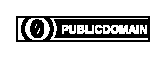
\includegraphics[height=6pt]{../cc-zero}}%
	\qquad%
	\insertframenumber{}/{}\inserttotalframenumber%
      \end{beamercolorbox}
    }
    \hbox{
      \begin{beamercolorbox}[wd=\paperwidth,ht=2.5ex,dp=1.125ex,leftskip=.3cm plus1fil,rightskip=.3cm]{author in head/foot}
	\usebeamerfont{author in head/foot}\insertshortauthor\hfill\insertshortinstitute
      \end{beamercolorbox}
    }
    \vskip0pt
  }
%   \addtobeamertemplate{frametitle}{}{
%     \begin{textblock*}{30mm}(.8\textwidth,-7mm)
%       \includegraphics[height=6mm,keepaspectratio]{figures/logo-fbk}
%       \hfill
%       \includegraphics[height=6mm,keepaspectratio]{figures/logo-ict}
%     \end{textblock*}
%   }
  \setbeamerfont*{itemize/enumerate body}{size=\normalsize}
  \setbeamerfont*{itemize/enumerate subbody}{size=\footnotesize,shape=\itshape}
%   \setbeamertemplate{frametitle}[shadow]
}

\AtBeginSection[]{
  \begin{frame}
  \vfill
  \centering
  \begin{beamercolorbox}[sep=8pt,center,shadow=true,rounded=true]{title}
    \usebeamerfont{title}\insertsectionhead\par%
  \end{beamercolorbox}
  \vfill
  \end{frame}
}

\newcommand{\email}[1]{\href{mailto:#1}{\nolinkurl{#1}}}
\DeclareRobustCommand{\todo}[1]{\ifdraft{\textbf{\textcolor{red}{[#1]}}}{}}
\newcommand{\citecustom}[2]{#2 (\citeyear{#1})}
\newcommand\credits[2][]{%
  \ifx&#1&%
  \def\x{}
  \else%
  \def\x{{#1}: }
  \fi%
  \begingroup%
  \renewcommand\thefootnote{}\footnote{{\x}{\textcopyright}#2}%
  \addtocounter{footnote}{-1}%
  \endgroup%
}
\def\newblock{\hskip .11em plus .33em minus .07em} %trick to avoid undefined command with bibtex
\def\randomSeed{1138}

\title{Ontologies\todo{40min}}
\author[Matthieu Vergne\qquad\email{matthieu.vergne@meritis.fr}]{
  \texorpdfstring{
    \textbf{Matthieu Vergne}
  }{Matthieu Vergne}
}
\institute[Meritis PACA]{
  Les Algorithmes - Aristote B\\
  2000 Route des Lucioles\\
  06901  Sophia Antipolis Cedex\\
  ~\\
  
\includegraphics[height=15mm,keepaspectratio]{../logo-meritis.jpg}
}
\date{TBD}

\begin{document}

\begin{frame}
\titlepage
\end{frame}

\begin{frame}
\frametitle{Outline}
\tableofcontents[hideallsubsections]
\end{frame}

\section{Introduction}
\subsection{}

\begin{frame}
\frametitle{Résumé}
\begin{itemize}
 \item \todo{}
\end{itemize}
\end{frame}

\section{Généralités}
\subsection{}

\begin{frame}
\frametitle{Objectifs d'une ontologie}
\begin{exampleblock}{Représentation + cohérence}
 Une ontologie définit des concepts et leurs relations.
 Une ontologie valide est une ontologie cohérente.
\end{exampleblock}
\begin{alertblock}{Les concepts et relations sont totalement arbitraires}
 Les méthodes de conceptions d'ontologies ne se préoccupe pas de savoir si les propriétés définies ont du sens.
 C'est au concepteur de l'ontologie de s'assurer que celle-ci représente bien son domaine.
\end{alertblock}
\end{frame}

\begin{frame}
\frametitle{Exemples d'ontologies}
Ontologies spécifiques :
\begin{itemize}
 \item Pizza : pizza, ingrédient, base, garniture, etc.\\
       {\scriptsize\url{https://protege.stanford.edu/ontologies/pizza/pizza.owl}}
 \item Automobile : véhicule, puissance, carburant, vitesse, etc.\\
       {\footnotesize\url{https://schema.org/docs/automotive.html}}
 \item Java : interface, variable, méthode, thread, etc.\\
       {\footnotesize\url{https://doi.org/10.1007/978-3-642-33642-3_16}}
\end{itemize}
Ontologies génériques (fondamentales) :
\begin{itemize}
 \item Dolce : parties, qualités, temps, espace, etc.\\
       {\footnotesize\url{http://www.loa.istc.cnr.it/dolce/overview.html}}
 \item UFO : types, roles, quantités, relations, etc.\\
       {\footnotesize\url{http://dev.nemo.inf.ufes.br/seon/UFO.html}}
\end{itemize}
\end{frame}

\section{Programmation de bibliothèque}
\subsection{}

\begin{frame}
\frametitle{Intérêt des ontologies}
Ontologies liées au domaine d'application :
\begin{itemize}
 \item Ontologies spécifiques fournissent des concept/relations pertinents à coder
 \item Ontologies génériques aident à abstraire
\end{itemize}
~\\
Pratiques ontologiques : \onslide<2->{\textcolor{red}{$\leftarrow$ focus de la présentation}}
\begin{itemize}
 \item Fournit des méthodes de conception génériques
 \item Permet de challenger le design de la bibliothèque
\end{itemize}
\end{frame}

\begin{frame}
\frametitle{Terminologie}
\begin{description}
 \item[Entité] Élément quelconque.\\
      {\footnotesize\textit{Ex: John, Mary}}
 \item[Propriété P] Attribut d'une entité.\\
      {\footnotesize\textit{Ex: John est une personne, John est marié à Mary}}
 \item[Instance de P] Entité ayant la propriété P.\\
      {\footnotesize\textit{Ex: John et Mary sont des instances de ``est une personne''}}
\end{description}
\begin{alertblock}{Instance ontologique $\neq$ instance Java}
 Pour la notion d'instance, on s'appuyera sur le contexte : instance d'une propriété vs. instance d'une classe.
\end{alertblock}
\end{frame}

\begin{frame}
\frametitle{Exemples Java}
\def\classA{\lstinline{Chat}\xspace}
\def\classB{\lstinline{Chien}\xspace}
\def\instA{\lstinline{kitty}\xspace}
\def\instB{\lstinline{rex}\xspace}
\def\field{\lstinline{nom}\xspace}
\begin{itemize}
 \item Les classes \classA et \classB définissent un champs \field
       \\$\rightarrow$ \classA et \classB ont la propriété ``définit un \field''
 \item \instA est une instance de \classA
       \\$\rightarrow$ \instA a les propriétés ``est un \classA'' + ``a un \field''
 \item \instB est une instance de \classB
       \\$\rightarrow$ \instB a les propriétés ``est un \classB'' + ``a un \field''
 \item ``a un \field'' est une propriété commune
       \\$\rightarrow$ \instA et \instB sont des instances de cette propriété
 \item ``est un \classA'' + ``a un \field'' = ``est un \classA nommé''
       \\$\rightarrow$ \instA a la propriété ``est un \classA nommé''
       \\$\rightarrow$ toute instance de \classA a la propriété ``est un \classA nommé''
\end{itemize}
\end{frame}

\begin{frame}
\frametitle{Points importants}
\begin{itemize}
 \item Une propriété peut être de n'importe quelle nature :
 \begin{itemize}
  \item être l'instance d'une classe
  \item définir un champs/une méthode
  \item avoir un champs à une valeur particulière
  \item implémenter une méthode particulière d'une interface
  \item combinaison d'autres propriétés
  \item etc.
 \end{itemize}
 \item Une propriété s'applique indépendamment des classes
 \begin{itemize}
  \item \lstinline{kitty} et \lstinline{rex} sont des instances de classes différentes, mais sont instances de la même propriété ``a un \lstinline{nom}''
 \end{itemize}
\end{itemize}
\end{frame}

\begin{frame}
\frametitle{Méta-propriétés}
\begin{itemize}
 \item Méta-propriété : propriété qui s'applique à une autre propriété
 \begin{itemize}
  \item Ex: ``est un \lstinline{Chat}'' est incompatible avec ``est un \lstinline{Chien}''
 \end{itemize}
 \item Ces méta-propriétés impactent la conception de bibliothèques
 \begin{itemize}
  \item Chaque incohérence d'une bibliothèque réduit sa réutilisabilité
 \end{itemize}
 \item Certaines méta-propriétés sont génériques
 \begin{itemize}
  \item Appliquables à n'importe quelle bibliothèque
 \end{itemize}
 \item Nous en couvriront 3 :
 \begin{description}
  \item[Rigidité] propriété essentielle d'une instance
  \item[Identité] propriété identifiant l'instance
  \item[Unité] propriété indécoupable
  \item \todo{Dépendance? Permanence? Réalité?}
 \end{description}
\end{itemize}
\end{frame}

\section{Rigidité}
\subsection{}

\begin{frame}
\frametitle{Définition}
\framesubtitle{\cite{goos_ontological_2000,staab_overview_2004}}
\begin{itemize}
 \item Une entité peut avoir des propriétés essentielles
 \begin{itemize}
  \item Ex. : John a nécessairement un cœur.
 \end{itemize}
 \item Une propriété essentielle ne change pas
 \begin{itemize}
  \item Ex. : le cœur de John peut être remplacé, mais il doit en avoir un.
 \end{itemize}
 \item Rigidité : propriété essentielle pour toutes ses instances
 \begin{itemize}
  \item Ex. : tout être humain doit forcément avoir un cœur.
 \end{itemize}
\end{itemize}
\end{frame}

\begin{frame}
\frametitle{Exemple Java}
\def\instance{\lstinline{i}\xspace}
\def\class{\lstinline{C}\xspace}
\def\prop{``est un \class''\xspace}
Instanciation d'une classe \class :
\begin{itemize}
 \item Une instance \instance de \class a la propriété \prop
 \item Cette propriété ne peut pas lui être retirée
 \begin{itemize}
  \item On ne peut que créer une nouvelle instance d'une autre classe
 \end{itemize}
 \item \prop est donc une propriété essentielle de \instance
 \item Toute entité avec cette propriété est une instance de \class
 \item Cette propriété est donc essentielle pour toutes ses instances
 \item \prop est donc une propriété rigide
\end{itemize}
~\\
Les propriétés statiques du langage sont rigides :
\begin{itemize}
 \item avoir un champs \lstinline{x} (imposée par la classe)
 \item avoir une méthode \lstinline{x()} (imposée par la classe)
 \item avoir un champs constant \lstinline{x=="foo"} (imposée par \lstinline{final})
 \item etc.
\end{itemize}
\end{frame}

\begin{frame}
\frametitle{Types de rigidité}
Une propriété peut être :
\begin{description}
 \item[Rigide] essentielle à toutes ses instances
 \item[Non-rigide] essentielle ou non, selon l'instance
 \item[Anti-rigide] essentielle pour aucune instance
\end{description}
~\\
Exemples de propriétés non-rigides :
\begin{itemize}
 \item avoir un champs de type \lstinline{Optional} vide
 \begin{itemize}
  \item Essentiel pour instance vide, pas pour instance muable
 \end{itemize}
 \item \lstinline{Supplier.get()} retourne \lstinline{"foo"}
 \begin{itemize}
  \item Essentiel si accesseur sur constante, pas sur champs muable
 \end{itemize}
\end{itemize}
~\\
Exemples de propriétés anti-rigides :
\begin{itemize}
 \item résultat de \lstinline{Random.nextInt()}
 \item contenu d'une file d'attente (e.g. \lstinline{Queue})
\end{itemize}
\end{frame}

\begin{frame}
\frametitle{Impacts}
\def\pa{$P$\xspace}
\def\pb{$P'$\xspace}
\def\ca{$\{P_i\}$\xspace}
\def\cb{$\{P'_i\}$\xspace}
\def\ia{$P_i$\xspace}
\def\ib{$P'_i$\xspace}
Contexte :
\begin{itemize}
 \item Étant donné une propriété \pa ayant des instances \ca
 \item Une sous-propriété \pb a des instances \cb $\subseteq$ \ca
\end{itemize}
~\\
Si \pa est non-rigide, \ia peut sortir ou non de \ca
\begin{itemize}
 \item \pb rigide (\cb fixe) ou non (\ib sort de \cb, voire de \ca)
\end{itemize}
Si \pa est rigide, \ia doit rester dans \ca
\begin{itemize}
 \item \pb rigide (\cb fixe) ou non (\ib sort de \cb, pas de \ca)
\end{itemize}
Si \pa est anti-rigide, \ia doit pouvoir sortir de \ca
\begin{itemize}
 \item \pb anti-rigide (\ib doit sortir de \cb pour sortir de \ca)
\end{itemize}
~\\
\begin{center}
 \textbf{$P$ anti-rigide $\Rightarrow$ $P'$ anti-rigide}
\end{center}
\end{frame}

\begin{frame}[fragile]
\frametitle{Exemple Java}
\def\Parent{Parent}
\def\Enfant{Enfant}
\begin{lstlisting}
class §\Parent§ {
  private String s;
  String getS() {return s;}
  void setS(String s) {this.s = s;}
}
class §\Enfant§ extends §\Parent§ {
  Enfant(String s) {super.setS(s);}
  void setS(String s) {throw new UnsupportedOperationException();}
}
\end{lstlisting}
\newcommand{\mathListing}[1]{\ensuremath{\text{\lstexpand{#1}}}}
\def\pa{\mathListing{x instanceof \Parent}}
\def\pb{\mathListing{x instanceof \Enfant}}
\def\pc{\mathListing{x.s="foo"}}
\def\pd{\ensuremath{\text{\lstinline{s} muable dans \lstexpand{\Parent}}}}
\def\pe{\ensuremath{\text{\lstinline{s} immuable dans \lstexpand{\Enfant}}}}
\only<1-2>{\small\begin{align*}
 &P(x) = \pa \wedge \pc \\
 &P'(x) = \pb \wedge \pc \\
 &\pb \Rightarrow \pa & \text{(héritage Java)} \\
 &P'(x) = P(x) \wedge \pb \Rightarrow P' \subset P \\
 &\pd \Rightarrow \text{$P$ anti-rigide} \Rightarrow \textbf<2>{\text{$P'$ anti-rigide}} & \text{(setter \lstexpand{\Parent})} \\
 &\pe \Rightarrow \textbf<2>{\text{$P'$ rigide}} \only<2>{\Rightarrow \text{contradiction}} & \text{(setter \lstexpand{\Enfant})} \\
\end{align*}
}
\only<3>{
\begin{alertblock}{Contradiction \emph{logique} : $P'$ ne peut être rigide et anti-rigide}
 \lstexpand{\Enfant} ne respecte pas l'anti-rigidité imposée par \lstexpand{\Parent}.
\end{alertblock}
\begin{itemize}
 \item Techniquement faisable : problème de design, pas de langage
 \item Problème observable à l'exécution :
 \begin{itemize}
  \item appel \lstinline{setS(s)} sur variable \lstexpand{\Parent} échoue si instance de \lstinline{Enfant}
 \end{itemize}
 \item  Bon design peut permettre contrôle à la compilation
\end{itemize}
}
\end{frame}

\begin{frame}
\frametitle{Solution}
\begin{exampleblock}{Ne pas être anti-rigide dès le départ}
 Penser non-rigide avant anti-rigide :
 \begin{itemize}
  \item parent abstrait + enfant 1 rigide + enfant 2 anti-rigide
  \item interface lecture, étendue avec écriture
  \item interface lecture + interface écriture (+ interface combinée)
 \end{itemize}
\end{exampleblock}
Problème présent de base en Java :
\begin{itemize}
 \item \lstinline{Collection} a un contenu variable (e.g. \lstinline{add}, \lstinline{remove})
 \begin{itemize}
  \item \lstinline{Collections.unmodifiableXxx(x)} et \lstinline{Arrays.asList(...)} l'empêchent (exceptions sur écriture)
 \end{itemize}
 \item \lstinline{Iterator} permet la suppression
 \begin{itemize}
  \item \lstinline{Iterator.remove(x)} génère une exception par défaut
 \end{itemize}
 \item Pas systématique :
 \begin{itemize}
  \item \lstinline{StringBuffer} = \lstinline{CharSequence} (lec.) + \lstinline{Appendable} (écr.)
  \item \lstinline{Supplier} (lec.) et \lstinline{Consumer} (écr.)
 \end{itemize}
\end{itemize}
\end{frame}

\section{Identité}
\subsection{}

\begin{frame}
\frametitle{Définition}
\framesubtitle{\cite{guarino_identity_2000}\todo{\cite{goos_ontological_2000,staab_overview_2004}}}
\begin{itemize}
 \item Une entité peut avoir des propriétés caractéristiques
 \begin{itemize}
  \item Ex. : numéro de sécurité sociale de John.
 \end{itemize}
 \item Une propriété caractéristique appartient à une seule instance
 \begin{itemize}
  \item Ex. : John est le seul à avoir ce numéro de sécurité sociale.
 \end{itemize}
 \item Une propriété caractéristique peut être de tout type
 \begin{itemize}
  \item Ex. : numéro unique, login + pass, nom + adresse + naissance, etc.
 \end{itemize}
 \item Identité : modèle de propriétés caractéristiques permettant de différencier chaque instance
 \begin{itemize}
  \item Ex. : chaque assuré est identifié par son numéro de sécurité sociale.
 \end{itemize}
 \item Une propriété porte une identité si toutes ses instances s'identifient de la même manière
 \begin{itemize}
  \item Ex. : la propriété ``assuré'' porte une identité par son ``numéro de sécurité sociale''.
 \end{itemize}
\end{itemize}
\end{frame}

\begin{frame}
\frametitle{Exemple Java}
\def\class{\lstinline{Véhicule}\xspace}
\def\prop{\lstinline{VIN}\xspace}
Identité d'un \class :
\begin{itemize}
%  \item \class est rigide : tout (non-)\class le reste\todo{utile ?}
 \item La classe \class a un champs \prop
 \begin{itemize}
  \item VIN (Vehicule Identification Number) ou numéro de série
 \end{itemize}
%  \item \prop n'existe dans aucune classe parente (e.g. \lstinline{Engin})
%  \begin{itemize}
%   \item Une tondeuse n'est pas un véhicule, et donc n'a pas de VIN
%  \end{itemize}
 \item Chaque \prop est unique : chaque \class a le sien
 \item La valeur de \prop est donc caractéristique de chaque instance
 \item \class porte donc une identité par son champs \prop
\end{itemize}
~\\
Quelques identités du langage :
\begin{itemize}
 \item \lstinline{Object} s'identifie par son emplacement mémoire (\lstinline{x == x})
 \item \lstinline{Integer} s'identifie par sa valeur (\lstinline{42 == 42})
 \item \lstinline{String} s'identifie par son contenu (\lstinline{"x" == "x"})
 \item etc.
\end{itemize}
\end{frame}

\begin{frame}
\frametitle{\lstinline{==} ou \lstinline{equals()} ?}
\begin{alertblock}{Java impose l'interprétation de \lstinline{==}}
 \begin{itemize}
  \item Il ne permet que de retrouver les même instances Java
  \item \small\lstinline{"x"=="x"} mais \lstinline{new String("x") != new String("x")}
 \end{itemize}
\end{alertblock}
\begin{exampleblock}{\lstinline{equals()} offre une équivalence redéfinissable}
 \begin{itemize}
  \item \lstinline{==} par défaut, modifiable pour chaque classe
  \item \scriptsize\lstinline{"x".equals("x")} et \lstinline{new String("x").equals(new String("x"))}
 \end{itemize}
\end{exampleblock}
\begin{block}{Recommandation : préférer \lstinline{equals()} plutôt que \lstinline{==}}
 \begin{itemize}
  \item Large utilisation et support de base
  \begin{itemize}
   \item \lstinline{List.equals(x)}, \lstinline{Arrays.equals(a, b)}, \lstinline{Set.add(x)}, \lstinline{Objects.equals(a, b)}, \lstinline{Predicate.isEqual(x)}, etc.
  \end{itemize}
  \item Dépendance des méchaniques internes
  \begin{itemize}
   \item Redéfinition \lstinline{equals()} $\Rightarrow$ redéfinition \lstinline{hashcode()}
  \end{itemize}
 \end{itemize}
\end{block}
\end{frame}

\begin{frame}
\frametitle{Exemple Java (révisé)}
Identités par \lstinline{==} révisées :
\begin{itemize}
 \item \lstinline{Object.equals()} basé sur son emplacement mémoire
 \item \lstinline{Integer.equals()} basé sur sa valeur
 \item \lstinline{String.equals()} basé sur son contenu
 \item etc.
\end{itemize}
~\\
Identités plus complexes :
\begin{itemize}
 \item \lstinline{Locale.equals()} basé sur ses champs langage, script, pays, variante et extensions (multiples données)
 \item \lstinline{Map.equals()} basé sur ses clés-valeurs (dynamique)
 \item \lstinline{List.equals()} sur ses éléments ordonnés (méta-donnée)
 \item etc.
\end{itemize}
\end{frame}

% \begin{frame}
% \frametitle{Types d'identité}
% Une identité peut être :
% \begin{description}
%  \item[équivalente] identité $\Leftrightarrow$ instance
%  \item[suffisante] identité $\Rightarrow$ instance
%  \item[nécessaire] identité $\Leftarrow$ instance
%  \item[inexistante] pas d'identité
% \end{description}
% ~\\
% Exemples d'identités suffisantes :
% \begin{itemize}
%  \item \todo{...}
% \end{itemize}
% Exemples d'identités nécessaires :
% \begin{itemize}
%  \item \todo{...}
% \end{itemize}
% Exemples d'identités inexistantes :
% \begin{itemize}
%  \item Aucun, tout a un emplamcement mémoire (``tout est \lstinline{Object}'')
% \end{itemize}
% \end{frame}

\begin{frame}
\frametitle{Impacts}
\def\pa{$P$\xspace}
\def\pb{$P'$\xspace}
\def\ca{$\{P_i\}$\xspace}
\def\cb{$\{P'_i\}$\xspace}
\def\ia{$P_i$\xspace}
\def\ib{$P'_i$\xspace}
\def\ea{$\chi$\xspace}
\def\eb{$\chi'$\xspace}
Contexte :
\begin{itemize}
 \item Étant donné une propriété \pa ayant des instances \ca
 \item Une sous-propriété \pb a des instances \cb $\subseteq$ \ca
\end{itemize}
~\\
Si \pa porte une identité \ea
\begin{itemize}
 \item Tous les \ca sont différenciables par \ea
 \item Tous les \cb sont donc aussi différenciables par \ea
 \item \pb porte donc forcément l'identité \ea
 \item \pb peut aussi porter une identité \eb spécifique
\end{itemize}
~\\
\begin{center}
 \textbf{$P$ porte identité $\chi$ $\Rightarrow$ $P'$ porte identité $\chi$}
\end{center}
\end{frame}

\begin{frame}[fragile]
\frametitle{Exemple Java}
\def\Parent{Parent}
\def\Enfant{Enfant}
\begin{lstlisting}
class Parent {  int a;
  public boolean equals(Object obj) {
    return ((Parent) obj).a == a;
  }
}
class Enfant extends Parent {  int b;
  public boolean equals(Object obj) {
    return super.equals(obj) && ((Enfant) obj).b == b;
  }
}
\end{lstlisting}
\newcommand{\mathListing}[1]{\ensuremath{\text{\lstexpand{#1}}}}
\def\pa{\mathListing{x instanceof \Parent}}
\def\pb{\mathListing{x instanceof \Enfant}}
\def\pd{\ensuremath{\text{\lstinline{a} différencie \lstexpand{\Parent}}}}
\def\pe{\ensuremath{\text{(\lstinline{a},\lstinline{b}) différencie \lstexpand{\Enfant}}}}
\only<1-2>{\small\begin{align*}
 &P(x) = \pa \\
 &P'(x) = \pb \Rightarrow P' \subset P & \text{(héritage Java)} \\
 &\text{$P$ porte identité \lstinline{a}} \Rightarrow \textbf<2>{\text{$P'$ porte identité \lstinline{a}}} & \text{(equals \lstexpand{\Parent})} \\
 &\text{$P'$ porte identité (\lstinline{a},\lstinline{b}) \only<2>{\textbf{mais plus \lstinline{a} seul}}} & \text{(equals \lstexpand{\Enfant})} \\
\end{align*}
}
\only<3>{
\begin{alertblock}{Contradiction \emph{logique} : $P'$ doit porter l'identité \lstinline{a}}
 \lstexpand{\Enfant} ne respecte pas l'identité imposée par \lstexpand{\Parent}.
\end{alertblock}
\begin{itemize}
 \item Techniquement faisable : problème de design, pas de langage
 \item Problème observable à l'exécution :
 \begin{itemize}
  \item \lstinline{parent.equals(enfant) != enfant.equals(parent)}
 \end{itemize}
 \item  Bon design peut permettre contrôle à la compilation
\end{itemize}
}
\end{frame}

\begin{frame}
\frametitle{Solution}
\begin{exampleblock}{Ne pas redéfinir le \lstinline{equals()} d'un parent instanciable}
 \begin{itemize}
  \item définir uniquement le \lstinline{equals()} du parent
  \item rendre le parent non-instanciable (constructeur non-public)
  \item composition plutôt qu'héritage
 \end{itemize}
\end{exampleblock}
Illustrations en Java :
\begin{itemize}
 \item \lstinline{AbstractList} le définit pour tous ses enfants
 \begin{itemize}
  \item \lstinline{ArrayList} et \lstinline{LinkedList} n'y touchent pas
 \end{itemize}
 \item \lstinline{Calendar} définit \lstinline{equals()} mais constructeur protégé
 \begin{itemize}\scriptsize
  \item \lstinline{GregorianCalendar} et \lstinline{JapaneseImperialCalendar} complètent
 \end{itemize}
 \item \small\lstinline{BigInteger.equals()} réutilisé par \lstinline{BigDecimal.equals()}
 \begin{itemize}
  \item Deux \lstinline{Number}, mais pas d'héritage entre les deux
 \end{itemize}
\end{itemize}
\end{frame}

\section{Unité}
\subsection{}

\begin{frame}
\frametitle{Définition}
\framesubtitle{\cite{goos_ontological_2000,staab_overview_2004}, \citecustom{noauthor_ontoclean_2019}{Wikipédia}}
\begin{description}
 \item[Unité] Une instance de la classe ne peut pas être décomposée en instances de la même classe.\\
      {\footnotesize\textit{Ex: statue d'argile (unité) vs. tas d'argile (\sout{unité})}}
\end{description}
\todo{...}
\end{frame}

\section{Impacts sur du code Java}
\subsection{}

\begin{frame}
\frametitle{Piège equals()}
\begin{itemize}
 \item Redéfinir equals() autrement que pour optimisation est une erreur.
\end{itemize}
\end{frame}

\begin{frame}
\frametitle{Piège override}
\begin{itemize}
 \item Seulement si fonctionnellement équivalent (e.g. optimisation, décoration)
\end{itemize}
\end{frame}

\begin{frame}
\frametitle{Piège "carré est un rectangle"}
\begin{itemize}
 \item Que des getters = OK
 \item Dès que setters = KO
\end{itemize}
Explication pour piège du equals() ?
\end{frame}

\begin{frame}[allowframebreaks]
\frametitle{Piège "id dans objet"}
\begin{itemize}
 \item ID n'existe que pour différencier plusieurs objets
 \item Propriété du contexte dans lequel l'objet se trouve, pas de l'objet lui-même
 \item Si changement de contexte, ID peut apparaître/disparaître/changer
 \item Exemple :
 \begin{itemize}
  \item contexte plus large impose ID plus grand
  \item typiquement concaténation (e.g. category-subcategory-instance)
  \item ID devrait pouvoir être infiniment grand/complété, jamais fixe
 \end{itemize}
\end{itemize}
\todo{Exemple commun : n° sécu, n° fiscal, n° passeport, n° téléphone, adresse e-mail, etc. représentent le même individu.
Un identifiant est un moyen simple d'identifier un individu, mais ce n'est pas une propriété essentielle de l'individu.
L'absence de ces identifiants n'implique pas l'absence de l'individu.
De plus, la multiplicité de ces identifiants met en lumière que l'identifiant dépend de la perspective prise sur l'individu.
Perspective sécu nécessite n° sécu, perspective fiscale n° fiscal, etc.
Tant qu'on se limite à une unique perspective, choisir de stocker l'ID dans l'objet représentant l'individu et de l'utiliser comme propriété d'identité est une question de choix de design.
Dès lors que cet objet doit être partagé entre plusieurs perspectives, ce choix devient une erreur de design.
De manière générale, il est préférable de ne pas stocker l'identifiant dans l'objet identifié, à moins de prendre l'hypothèse volontaire que cet objet n'existera que dans une unique perspective.}
\end{frame}

\section{Conclusion}
\subsection{}

\begin{frame}
\frametitle{Points importants}
\begin{itemize}
 \item \todo{}
\end{itemize}
\todo{Autre méta-propriété : dépendance.
L'existence de l'instance présuppose l'existence d'une autre instance.
Ex: un étudiant a forcément un professeur.
Notion peu claire, donc non décrite ici, mais à étudier pour voir si utile.}
\todo{\cite{welty_towards_2005} ajoute les méta-propriétés permanence et réalité (actuality en anglais).}
\end{frame}

\begin{frame}
\frametitle{Aller plus loin}
\todo{Autre méta-propriété : dépendance.
L'existence de l'instance présuppose l'existence d'une autre instance.
Ex: un étudiant a forcément un professeur.
Notion peu claire, donc non décrite ici, mais à étudier pour voir si utile.}
\todo{\cite{welty_towards_2005} ajoute les méta-propriétés permanence et réalité (actuality en anglais).}
\end{frame}

\appendix
\newcounter{finalframe}
\setcounter{finalframe}{\value{framenumber}}

\begin{frame}[allowframebreaks]{Bibliography}
\bibliographystyle{plainnat-fr}
\bibliography{bibliography}
\end{frame}

\setcounter{framenumber}{\value{finalframe}}
\end{document}
